\documentclass[a4paper,10pt,twocolumn]{article}
\usepackage[utf8]{inputenc}
\usepackage{amsmath, amssymb}
\usepackage{tcolorbox}
\tcbuselibrary{breakable}
\usepackage[margin=0.3in]{geometry}
\usepackage{array,epsfig}
\usepackage{centernot}
\usepackage{amsfonts}
\usepackage{amsxtra}
\usepackage{amsthm}
\usepackage{mathrsfs}
\usepackage{color}
\usepackage{algorithm}
\usepackage{algpseudocode}
\usepackage{tikz}
\usetikzlibrary{calc, decorations.pathmorphing, decorations.pathreplacing, decorations.shapes} 

\usepackage{enumitem}
\setlist[itemize]{itemsep=0pt, parsep=0pt, left=2pt, topsep=0pt, labelsep=2pt, label=$\cdot$}

\makeatletter
\g@addto@macro\normalsize{
    \setlength{\abovedisplayskip}{2pt}
    \setlength{\belowdisplayskip}{2pt}
    \setlength{\abovedisplayshortskip}{2pt}
    \setlength{\belowdisplayshortskip}{2pt}
}
\makeatother

\pagestyle{empty}
\raggedbottom

\tcbset{
    module/.style={
        colback=white,
        colframe=black,
        fonttitle=\bfseries\scriptsize,
        fontupper=\scriptsize,
        boxrule=0.4pt,
        arc=1mm,
        outer arc=1mm,
        colbacktitle=gray!20,
        coltitle=black,
        boxsep=0.5mm,
        left=0.5mm, right=0.5mm, top=0.5mm, bottom=0.5mm,
        breakable
    },
}

\begin{document}

\twocolumn[
    \begin{center}
        \textbf{\footnotesize CS 171 F24 Final Exam Reference Sheet} \\
        \textit{\scriptsize Created by Steven He, 2024}
    \end{center}
]

\vspace{-1em}

\begin{tcolorbox}[title=Uninformed Search, module]
    A \textbf{state} represents particular configuration of environment. \textbf{Nodes} in search tree can encode details like state, parent, action, path cost, depth, etc.

    \textbf{Tree Search} doesn't remember visited nodes: slow search, low memory
    \textbf{Graph Search} remembers visited nodes: fast search, high memory

    Basic search scheme maintains explored and frontier nodes. Process the frontier in some order based on some policy/search strategy, marking as visited if graph search, then expanding node.

    \textbf{Strategies evaluted by:}
    \begin{itemize}
        \item \textit{completeness} - does it guarantee a solution if one exists
        \item \textit{optimality} - does it guarantee min-cost solution
        \item \textit{time/space complexity} - \# of nodes generated / max \# of nodes in memory. In terms of max branching factor $b$, depth of min-cost solution $d$, maximum depth of state space $m$.
    \end{itemize}

    \textbf{Uninformed search strategies:}
    \begin{itemize}
        \item \textit{Breadth-first Search} - Frontier is FIFO queue. Goal test node before push. Always complete; only optimal if cost is non-decreasing function of depth.
        \item \textit{Uniform-cost Search} - Frontier is priority queue, ordered by total path cost $g(n)$. Goal test after popping from queue. Complete if $b$ is finite; optimal if all step costs $\ge \epsilon > 0$ (non-zero).
        \item \textit{Depth-first Search} - Frontier is LIFO stack. Defined as Depth-limited search with limit $l = \infty$. Goal test after pop from stack. Incomplete if depth of states is infinite; not optimal.
        \item \textit{Iterative Deepening Search} - Perform Depth-limited search, while iteratively increasing depth limit. Memory advantage of DFS, completeness \& optimality conditions of BFS.
    \end{itemize}

\end{tcolorbox}


\begin{tcolorbox}[title=Heuristic Search, module]
    A \textit{heuristic} estimates best possible cost left to the solution, denoted as $h(n)$.

    \vspace{-1em}
    \[
        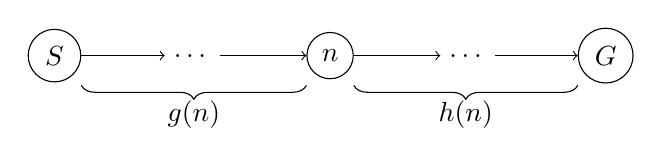
\begin{tikzpicture}[node distance=2cm, auto]
            \node[circle, draw, minimum size=0.5cm] (S) {$S$};
            \node[circle, draw, minimum size=0.5cm, right of=S, xshift=1.5cm] (n) {$n$};
            \node[circle, draw, minimum size=0.5cm, right of=n, xshift=1.5cm] (G) {$G$};

            \draw[->] (S) -- ($(S)!0.4!(n)$);
            \node at ($(S)!0.5!(n)$) {\ldots};
            \draw[->] ($(S)!0.6!(n)$) -- (n);

            \draw[->] (n) -- ($(n)!0.4!(G)$);
            \node at ($(n)!0.5!(G)$) {\ldots};
            \draw[->] ($(n)!0.6!(G)$) -- (G);

            \draw [decorate,decoration={brace,amplitude=5pt,mirror,raise=2.5ex}]
            ($(S.east)!0!(n.west)$) -- ($(S.east)!1!(n.west)$) 
            node[midway,yshift=-3em] {$g(n)$};
            
            \draw [decorate,decoration={brace,amplitude=5pt,mirror,raise=2.5ex}]
            ($(n.east)!0!(G.west)$) -- ($(n.east)!1!(G.west)$)
            node[midway,yshift=-3em] {$h(n)$};
        \end{tikzpicture}
    \]
    \vspace{-1em}
    \[
        \begin{aligned}
            g(n) &: \text{known path cost so far to state } n \\
            h(n) &: \text{estimate of optimal cost to goal from } n \\
            f(n) = g(n) + h(n) &: \text{estimate of total cost to goal through } n \\
        \end{aligned}
    \]

    A heuristic is \textbf{admissible} iff $\forall n, h(n) \le h^*(n)$, where $h^*(n)$ is true optimal cost to goal. Admissible heuristics never overestimate cost to the goal.

    A heuristic is \textbf{consistent} iff $\forall n, f(n') \ge f(n)$ where $n'$ is any successor of $n$. $f(n)$ is non-decreasing along any path.

    \vspace{-1em}
    \[
        \begin{aligned}
            \textbf{consistent} &\implies \textbf{admissible} \\
            \neg \textbf{admissible} &\implies \neg \textbf{consistent} \\
            \textbf{admissible} &\centernot \implies \textbf{consistent} \\
        \end{aligned}
    \]

    \textbf{Heuristic search strategies:}
    \begin{itemize}
        \item \textit{Greedy Best-first Search} - Frontier is priority queue, ordered by heuristic $h(n)$. Only graph version complete in finite spaces; not optimal even with perfect heuristic $h = h^*$.
        \item $A^*$\textit{Search} - Frontier is priority queue, ordered by heuristic + path cost $f(n)$. Complete unless infinite nodes with $f < f(G)$. Optimal with tree search if $h$ is admissible; graph search if $h$ is consistent.
    \end{itemize}

    For two heuristics, if $\forall n, h_2(n) \ge h_1(n)$ then $h_2$ \textbf{dominates} $h_1$. If $h_2$ dominates $h_1$ and both are admissible, then $h_2$ is almost always better, and never expands more nodes than $h_1$.

    A problem with fewer restrictions is called \textbf{relaxed} (add more available actions). The solution of a relaxed problem is at least as good as the solution for the original problem. Intuition: If original problem hard to solve, relax the problem state space that is easy to solve. Solve it exactly and use the solution as heuristic for original problem.

    \textbf{Thm. } Heuristics that are generated from relaxed models are consistent

    \vspace{-0.5em}
    \[\textbf{Local Search}\]
    In some problems, path is irrelevant so we might avoid systematic search. The goal state itself is the solution.

    \textbf{Random restart wrapper} - Repeatedly perform local search, each time starting from a new random start state

    \textbf{Tabu search wrapper} - Within each random restart, add visited states to a "tabu" list of states that are temporarily excluded from being revisited.

    \textbf{Local search algorithms:}
    \begin{itemize}
        \item \textit{Hill Climbing} - At some current state, always compare to neighboring state with maximum value. If current state has better value, return, otherwise set current to the best neighbor. Neither complete nor optimal since we always approach local and not global optima relative to current position.
        \item \textit{WalkSAT} - Starting from random assignment, instead of always picking neighbor with most satisfied clauses, with some probability $p$, flip a random symbol (pick random neighbor). Randomness can potentially help escape local optima.
        \item \textit{Local Beam Search} - Create $k$ random initial states, generate their children, then select $k$ best children. Repeat until goal found.
        \item \textit{Simulated Annealing} - Intelligently combine random and greedy moves. Some temperature $T$ gradually decreases, representing state volatility. Temperature gives probability of forcing a random move.
        \item \textit{Genetic ALgorithms} - Mimic biology by mutating some set of offspring by crossing over traits, and selecting individuals based on fitness (heuristic) function.
    \end{itemize}

\end{tcolorbox}

\begin{tcolorbox}[title=Game Search, module]
    \textbf{todo}
\end{tcolorbox}

\begin{tcolorbox}[title=Constraint Satisfaction, module]
    \textbf{todo}
\end{tcolorbox}

\begin{tcolorbox}[title=Logic, module]
    \textbf{todo}
\end{tcolorbox}

\begin{tcolorbox}[title={Probability \& Uncertainty, Bayesian Networks}, module]
    \textbf{todo}
\end{tcolorbox}

\begin{tcolorbox}[title={Intro to ML, Linear Regression, kNN}, module]
    \textbf{todo}
\end{tcolorbox}

\begin{tcolorbox}[title={Decision Trees and Neural Networks}, module]
    \textbf{todo}
\end{tcolorbox}

\begin{tcolorbox}[title={Reinforcement Learning}, module]
    \textbf{Markov Property} - Future is independent of past given present:
    \[
        \mathbb{P}[S_{t + 1} | S_t] = \mathbb{P}[S_{t + 1} | S_1, \ldots, S_t] \text{ where } S_t \text{ is state at time } t
    \]

    We use matrix $\mathcal{P}$ to define transition property from state $s$ to $s'$, denoted as probability in row $s$, column $s'$.
    \[
        \mathcal{P} =
        \begin{bmatrix}
            \mathcal{P}_{11} & \ldots & \mathcal{P}_{1n} \\
            \vdots & \ddots & \vdots \\
            \mathcal{P}_{n1} & \ldots & \mathcal{P}_{nn} \\
        \end{bmatrix}
        , \mathcal{P}_{ss'} = \mathbb{P}[S_{t+1} = s' | S_t = s]
    \]

    \textbf{Markov Process/Chain} - Sequence of states $S_1, S_2, \ldots$ satisfying Markov property. Formally defined as tuple $\langle \mathcal{S}, \mathcal{P} \rangle$ i.e. (set of states, prob matrix)

    \textbf{Episode} - Some sequence of traveresed states in a MP

    \textbf{Markov Reward Process} - Give states in MP some reward. We ``gain'' reward $R_{t + 1}$ when transitioning from states $S_t \to S_{t + 1}$

    placeholder intermediary stuff goes here

    \[
        \begin{tabular}{|c|c|c|}
            \hline
            & \textbf{Evaluate Policy, $\pi$} & \textbf{Find Best Policy, $\pi^*$} \\
            \hline
            \textbf{MDP Known} & Policy Evaluation & Policy/Value Iteration \\
            \textbf{(Planning probs)} && \\
            \hline
            \textbf{MDP Unknown} & MC and TD Learning & Q-Learning \\
            \hline
        \end{tabular}
    \]

\end{tcolorbox}

\end{document}
